\chapter{Event Reconstruction and Selection}
\label{chap:objects}

\section{Introduction}

The CMS \Hgg analysis is able to perform measurements of Higgs boson properties using the diphoton invariant mass distribution.
Photon pairs resulting from Higgs decays produce a narrow signal peak, centred at the value of the Higgs mass, in this distribution.
This can be measured on top of the smoothly falling background distribution, produced by other SM processes.
The Higgs mass is inferred from two photons by constructing the diphoton invariant mass, which is given by the following expression
\begin{equation}
\mgg = \sqrt{ 2 E_{\gamma_1} E_{\gamma_2} (1 - \cos{\theta}) }
\end{equation}
where $E_{\gamma_1}$ and $E_{\gamma_2}$ are the energies of each photons, and $\theta$ is the opening angle between them.
The sensitivity of the analysis is maximised when the diphoton mass resolution is reconstructed as precisely as possible.
This requires the two photons to be correctly identified and their positions and energies accurately measured.
Furthermore, the location of the interaction vertex from which the photons originated must be established in order to calculate the opening angle.
Additional objects in the event, including jets and leptons, are further used to improve the sensitivity of the analysis and measure different Higgs production processes.

This section describes the official CMS procedure for reconstructing physics objects using the particle flow algorithm \cite{ParticleFlow}.
In addition, the photon and vertex identification techniques specific to the \Hgg analysis are detailed.
The approach used is almost identical between the 2016 and 2017 datasets; 
any differences are highlighted in the text.
%TODO consider adding an appendix for machine learning/BDTs?

\section{Particle flow}
The global event description at CMS is formed using the particle-flow algorithm (PF).
The goal of PF is to optimally combine the information of all the CMS subdetectors, 
enabling the best possible identification and energy measurements for all types of objects.
Inputs to the PF algorithm are tracks from originating from the tracker and muon system, 
and calorimeter clusters from the ECAL and HCAL.
CMS is able to benefit from the PF approach due to its strong magnetic field, 
alongside the fine segmentation and hermeticity of the tracker, calorimeters, and muon system.
Together these allow different types of objects to be separately identified, 
and the energy measurement to come from the subdetector with the best resolution.

Tracks are reconstructed from hits in the tracker using multiple iterations of a combinatorial track-finding procedure \cite{TrackReco}.
Each iteration proceeds in the following way.
First, track seeds comprising of two or three hits are chosen, defining the initial track parameters.
Then an extrapolation is performed along the expected track paths, adding any additional hits consistent with the path hypothesis.
Next the track parameters are re-estimated, and the track candidate collection is pruned based on quality criteria.
All the selected hits are then removed from consideration in the following iterations.
In this way, the first iteration identifies the most obvious tracks, normally those with high \pt and near to the interaction point.
The complexity of the subsequent iteration is reduced since many hits have been removed
This therefore permits lower thresholds to be used and lower \pt or highly displaced tracks to be found.
Additionally, muon tracks are constructed independently from hits in the muon system.

In the calorimeters, a clustering algorithm is used to collect together energy deposits belonging to each shower. %no clustering in HF
The procedure in the ECAL is described here, since it is an important input to the \Hgg analysis; the HCAL procedure is similar.
The clustering algorithm begins by selecting cluster seeds, which have an energy above a threshold and higher than any neighbouring crystal.
So-called topological clusters are then constructed iteratively by adding deposits which share a side or corner with one already in the cluster, 
provided their energy exceeds a threshold dependent on the noise level. %extra E_T requirement in the endcaps
If a crystal could be included in more than one topological cluster, its energy is shared between them assuming a Gaussian shower shape.
Finally, topological clusters are grouped into so-called superclusters (SCs).
This step is designed to recover energy lost via bremsstrahlung; 
radiated showers typically have the same $\eta$ but are spread in $\phi$ by the magnetic field.

Given these tracks and calorimeter clusters as inputs, the particle flow algorithm forms collections of candidates for five types of particle:
\begin{itemize}
  \item{\textbf{Muons:} a path extrapolated from the tracker is consistent with a muon track. 
                        The energy is inferred from the curvature of the track.} %actually uses muon info too when pT > 200 GeV.
  \item{\textbf{Electrons:} an ECAL SC is present and associated with a track from the inner tracker. 
                            The energy is measured using a combination of the track \pt and the SC energy.}
  \item{\textbf{Photons:} an ECAL SC is present and no track is associated with it.
                          The energy is measured using the ECAL SC only.}
  \item{\textbf{Neutral hadrons:} matched ECAL and HCAL clusters with no associated track.
                                 Energy measurement is the sum of the cluster energies.}
  \item{\textbf{Charged hadrons:} a track is matched to ECAL and HCAL clusters.
                                 The track curvature is used together with the calorimeter deposits to calculate the energy.}
\end{itemize}
In this way, the central CMS software provides analyses with physics objects ready for analyses.
The remainder of this chapter describes how these objects are used in the \Hgg analysis.

\section{Samples}
\subsection{Data}
\subsection{Simulation}

\section{Photon reconstruction}

Photons to be used in the \Hgg analysis are selected from the PF list of photon candidates.
A correction is then made to the SC energy using a multivariate regression technique.
After that, data and MC are brought into agreement by applying additional scale and smearing corrections to the photon energies.
A set of pre-selection criteria is applied to obtain the final set of photons considered in the analysis.
One of these criteria is a cut on the output score of the photon identification BDT, 
which is trained to reduce the contamination from other objects which mimic real photons.

Different types of variables are used to perform these steps.
They can be divided into shower shape and isolation variables.
The ECAL shower shape information is used both to correct the energy and discriminate between real and fake photons.
Isolation variables can be used to reduce the mis-identification of jets and other objects imitating a real photon signal.
The full set of variables used in this section and their definitions are given below.
\\ \\
\textbf{Shower shape variables:}
\begin{itemize}[noitemsep]
\item \emph{$E_{2\times2}/E_{5\times5}$}: the ratio of the energy in the 2x2 grid
  containing the most energetic cells in the SC to the energy in
  the 5x5 grid centered on the SC seed.
\item \emph{$cov_{i\eta i\phi}$}: the covariance of the single crystal $\eta$
  and $\phi$ values in within the 5x5 grid centered on the
  SC seed.
\item \emph{$\sigma_{i\eta i\eta}$}: the standard deviation 
  shower in terms of number of crystal cells. 
\item \emph{$\RNINE$}: $E_{3x3}/E_{SC}$ where $E_{3x3}$ is the energy sum of the
  3x3 grid surrounding the SC seed and $E_{SC}$ is the energy sum of the SC. 
\item \emph{$\sigma_{\eta}$}: the standard deviation
  of single crystal $\eta$ values within the SC, weighted by the logarithm of the crystal energy.
\item \emph{$\sigma_{\phi}$}: the standard deviation
  of single crystal $\phi$ values within the SC, weighted by the logarithm of the crystal energy.
\item \emph{Preshower $\sigma_{RR}$}: the standard deviation of the shower
  spread in the x-y plane of the preshower detector (endcap only).
\end{itemize}

\textbf{Isolation variables:}
\begin{itemize}[noitemsep]
\item H/E: the ratio of the energy in the HCAL cells behind the SC
  and the SC energy.
\item \emph{$\mathcal{I}_{\text{ph}}$}: 
  photon isolation,
  defined as the sum of the transverse energy of the particles
  identified as photons falling inside a cone of radius
  $R=0.3$
  around the photon candidate direction.
\item \emph{$\mathcal{I}_{\text{tk}}$}: 
  track isolation in a hollow cone
  the sum of the transverse momenta
  of all tracks in a cone of radius $R=0.3$
  around the photon candidate direction (with tracks in an
  inner cone of size $R=0.04$ not included in the sum).
  %the cone is hollow because the isolation definition is 
  %also used for electrons, and the track from the electron
  %itself is excluded;
\item \emph{$\mathcal{I}_{\text{ch}}$}: 
  charged hadron isolation,
  the sum of the transverse momenta of
  charged particles inside a cone of radius $R<0.3$ around the
  photon candidate.
\end{itemize}

\textbf{Miscellaneous:}
\begin{itemize}[noitemsep]
\item \emph{Electron veto}: rejects the photon candidate if its 
         supercluster is matched to an electron track.
\item \emph{$\rho$}: the median energy  density per unit area in the event.
\item \emph{$E_{SC}$}: the raw energy of the supercluster
  corresponding to the reconstructed photon, before corrections.
\end{itemize}

\subsection{Photon energy}
\subsection{Photon pre-selection}
\subsection{Photon identification}

\begin{figure}[h!]
  \centering
  \begin{subfigure}{0.45\textwidth}
    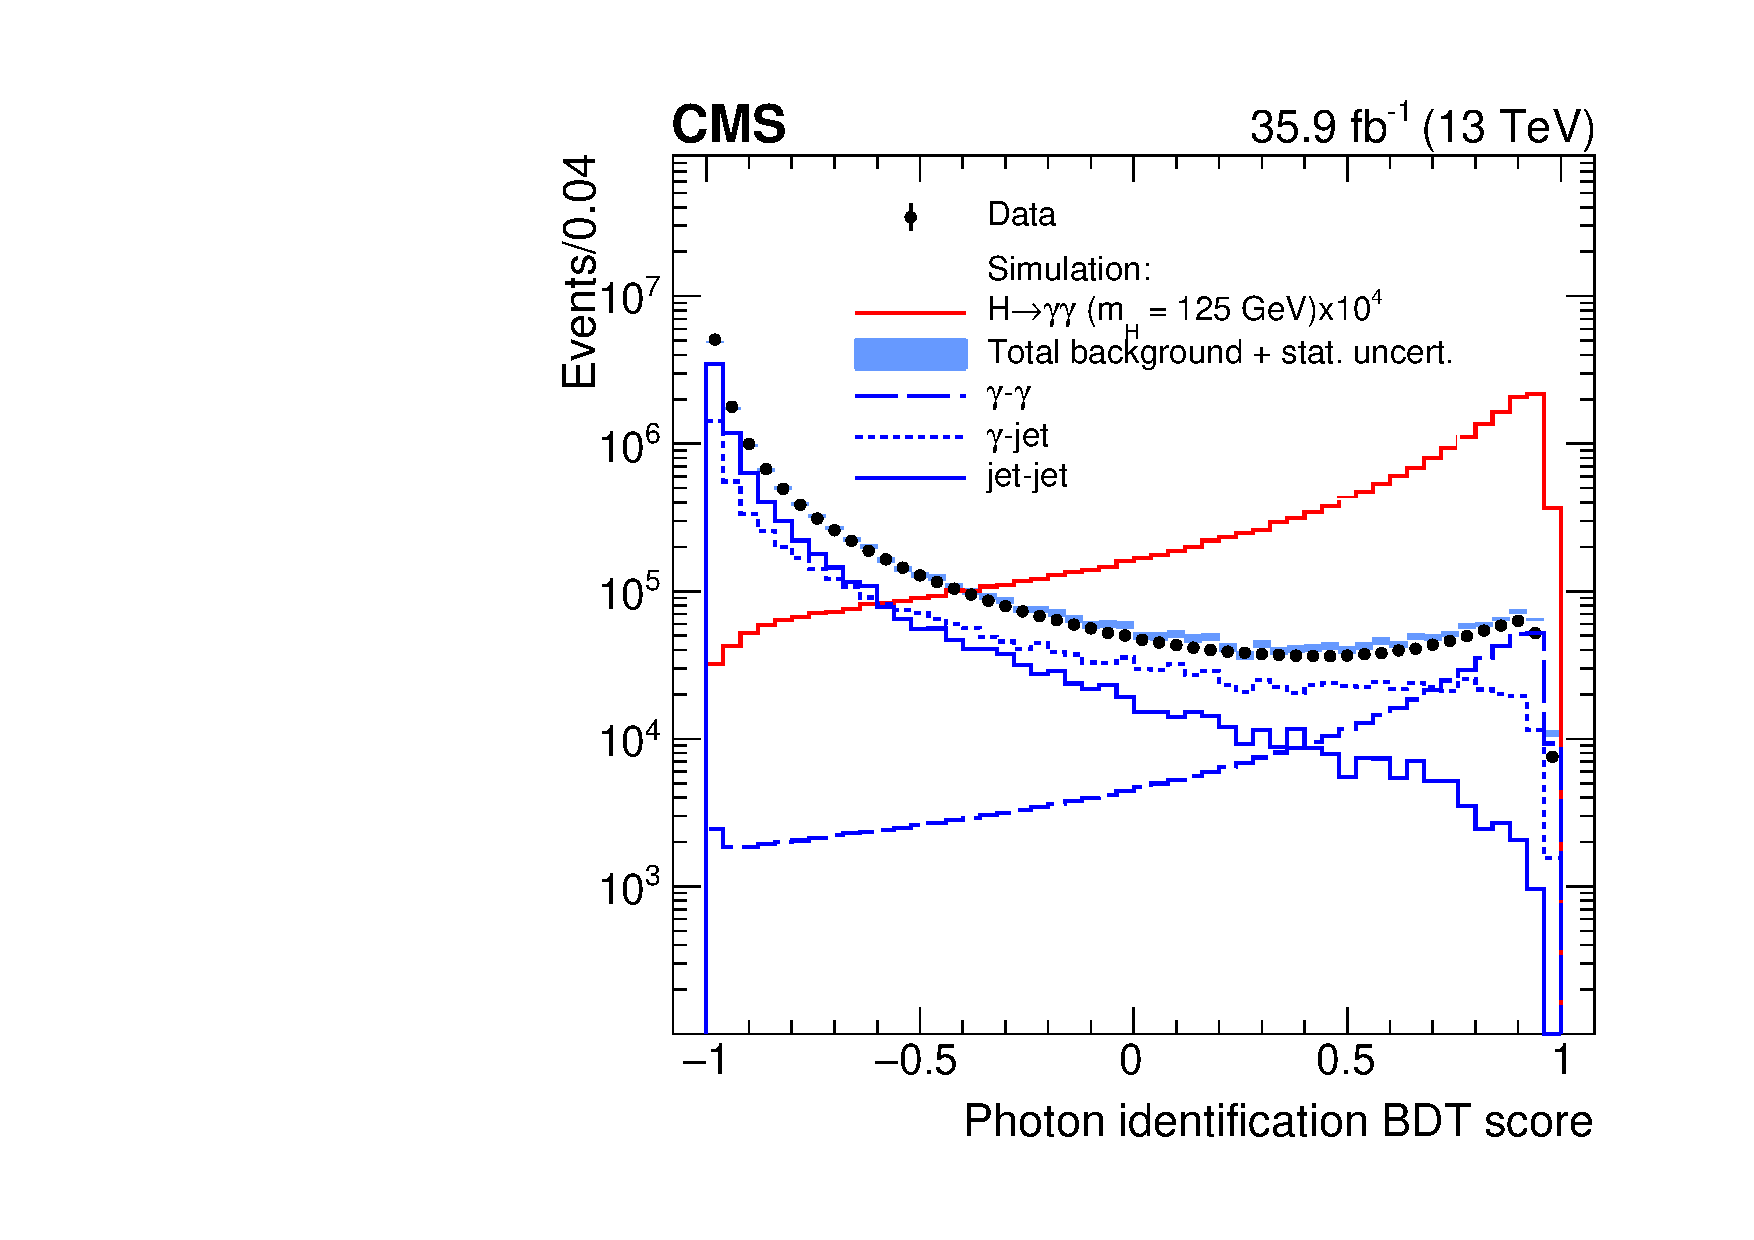
\includegraphics[width=\textwidth]{Figures/Objects/IDMVA_2016}
    \caption{2016}
    \label{fig:obj_IDMVA_2016}
  \end{subfigure}
  \begin{subfigure}{0.45\textwidth}
    \includegraphics[width=\textwidth]{Figures/Objects/IDMVA_2017}
    \caption{2017}
    \label{fig:obj_IDMVA_2016}
  \caption{Distribution of the photon identification BDT score of the lowest scoring photon
  of diphoton pairs with an invariant mass in the range $100 < \mgg < \SI{180}{GeV}$, for events passing
  the preselection in the 13 TeV data set (points), and for simulated background events (blue
  histogram). Histograms are also shown for different components of the simulated background.
  The sum of all background distributions is scaled up to data. The red histogram corresponds
  to simulated Higgs boson signal events}
  \label{fig:obj_IDMVA}
  \end{subfigure}
\end{figure}

\begin{figure}[h!]
  \centering
  \begin{subfigure}{0.45\textwidth}
    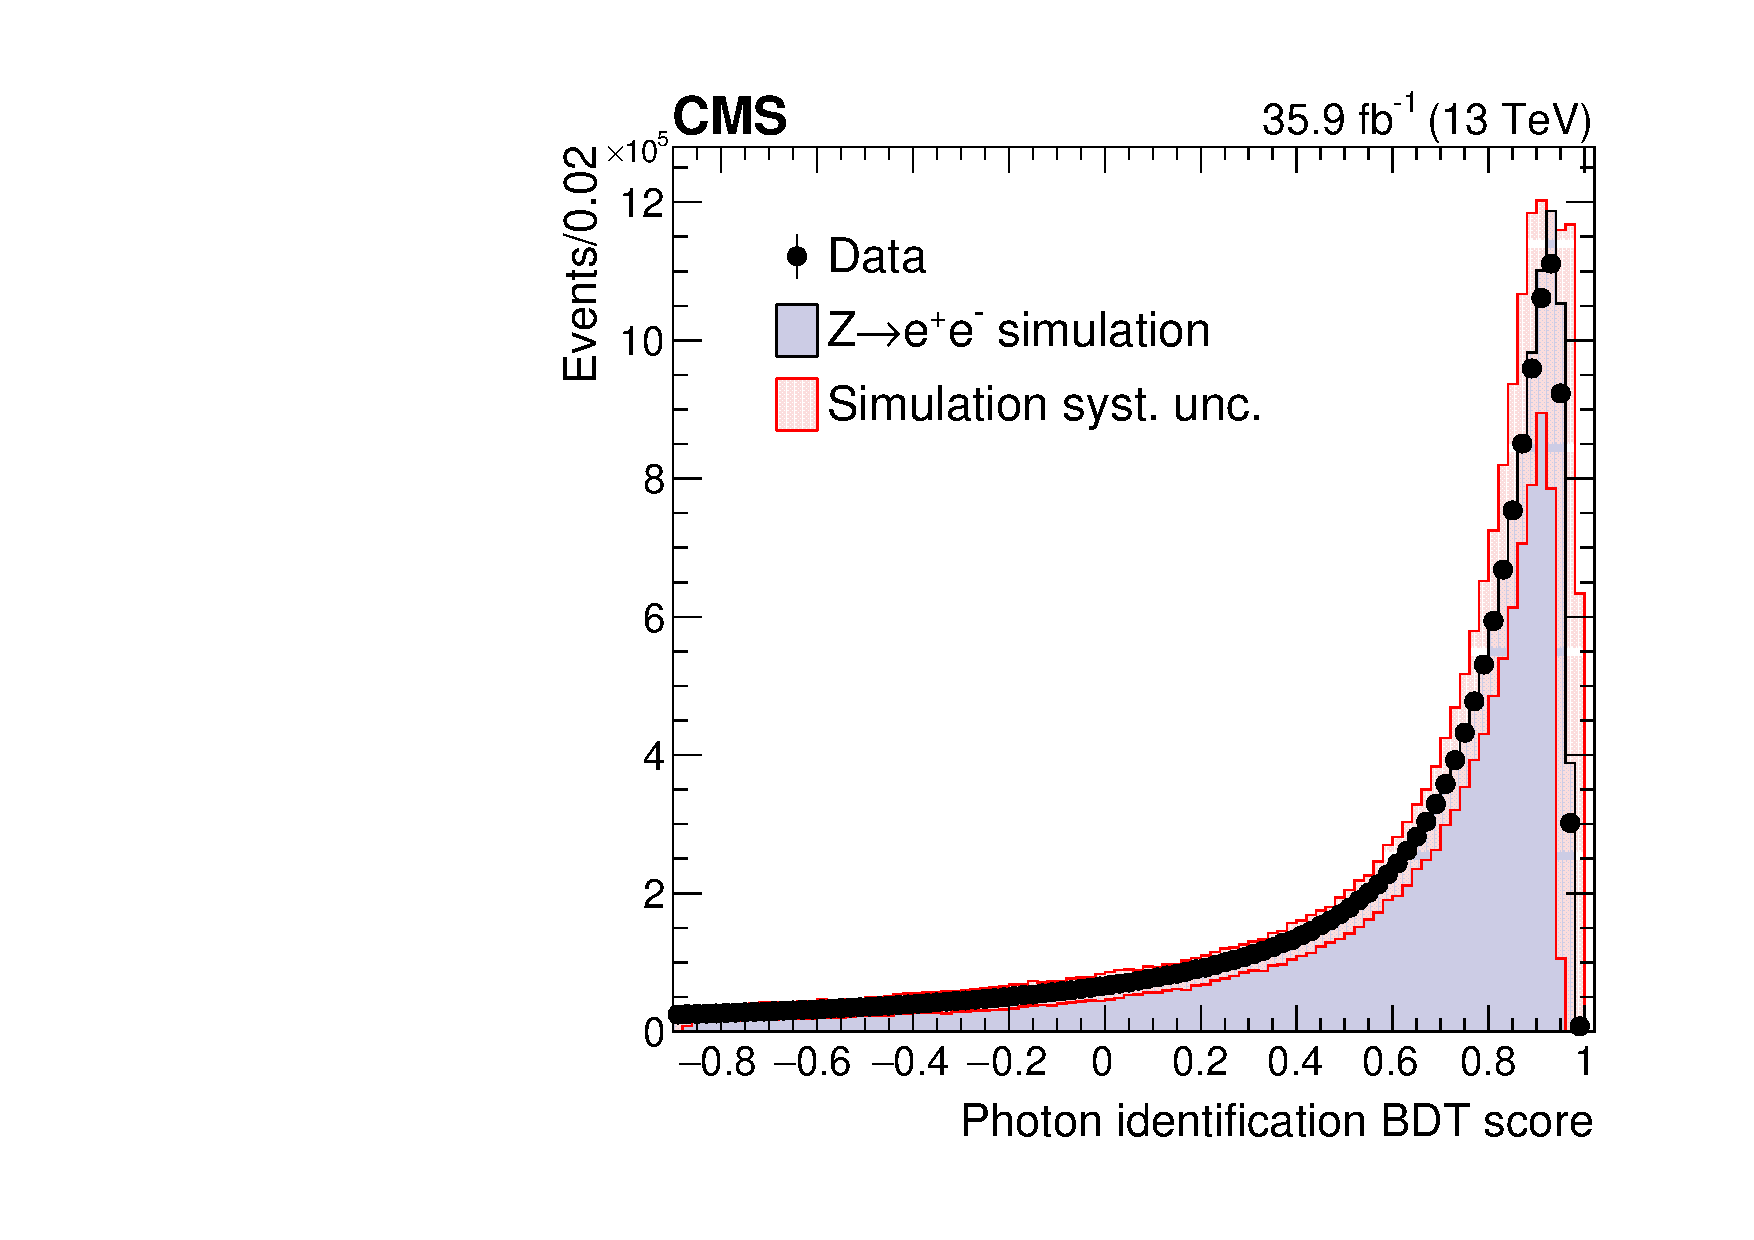
\includegraphics[width=\textwidth]{Figures/Objects/IDMVAZee_2016}
    \caption{2016}
    \label{fig:obj_IDMVAZee_2016}
  \end{subfigure}
  \begin{subfigure}{0.45\textwidth}
    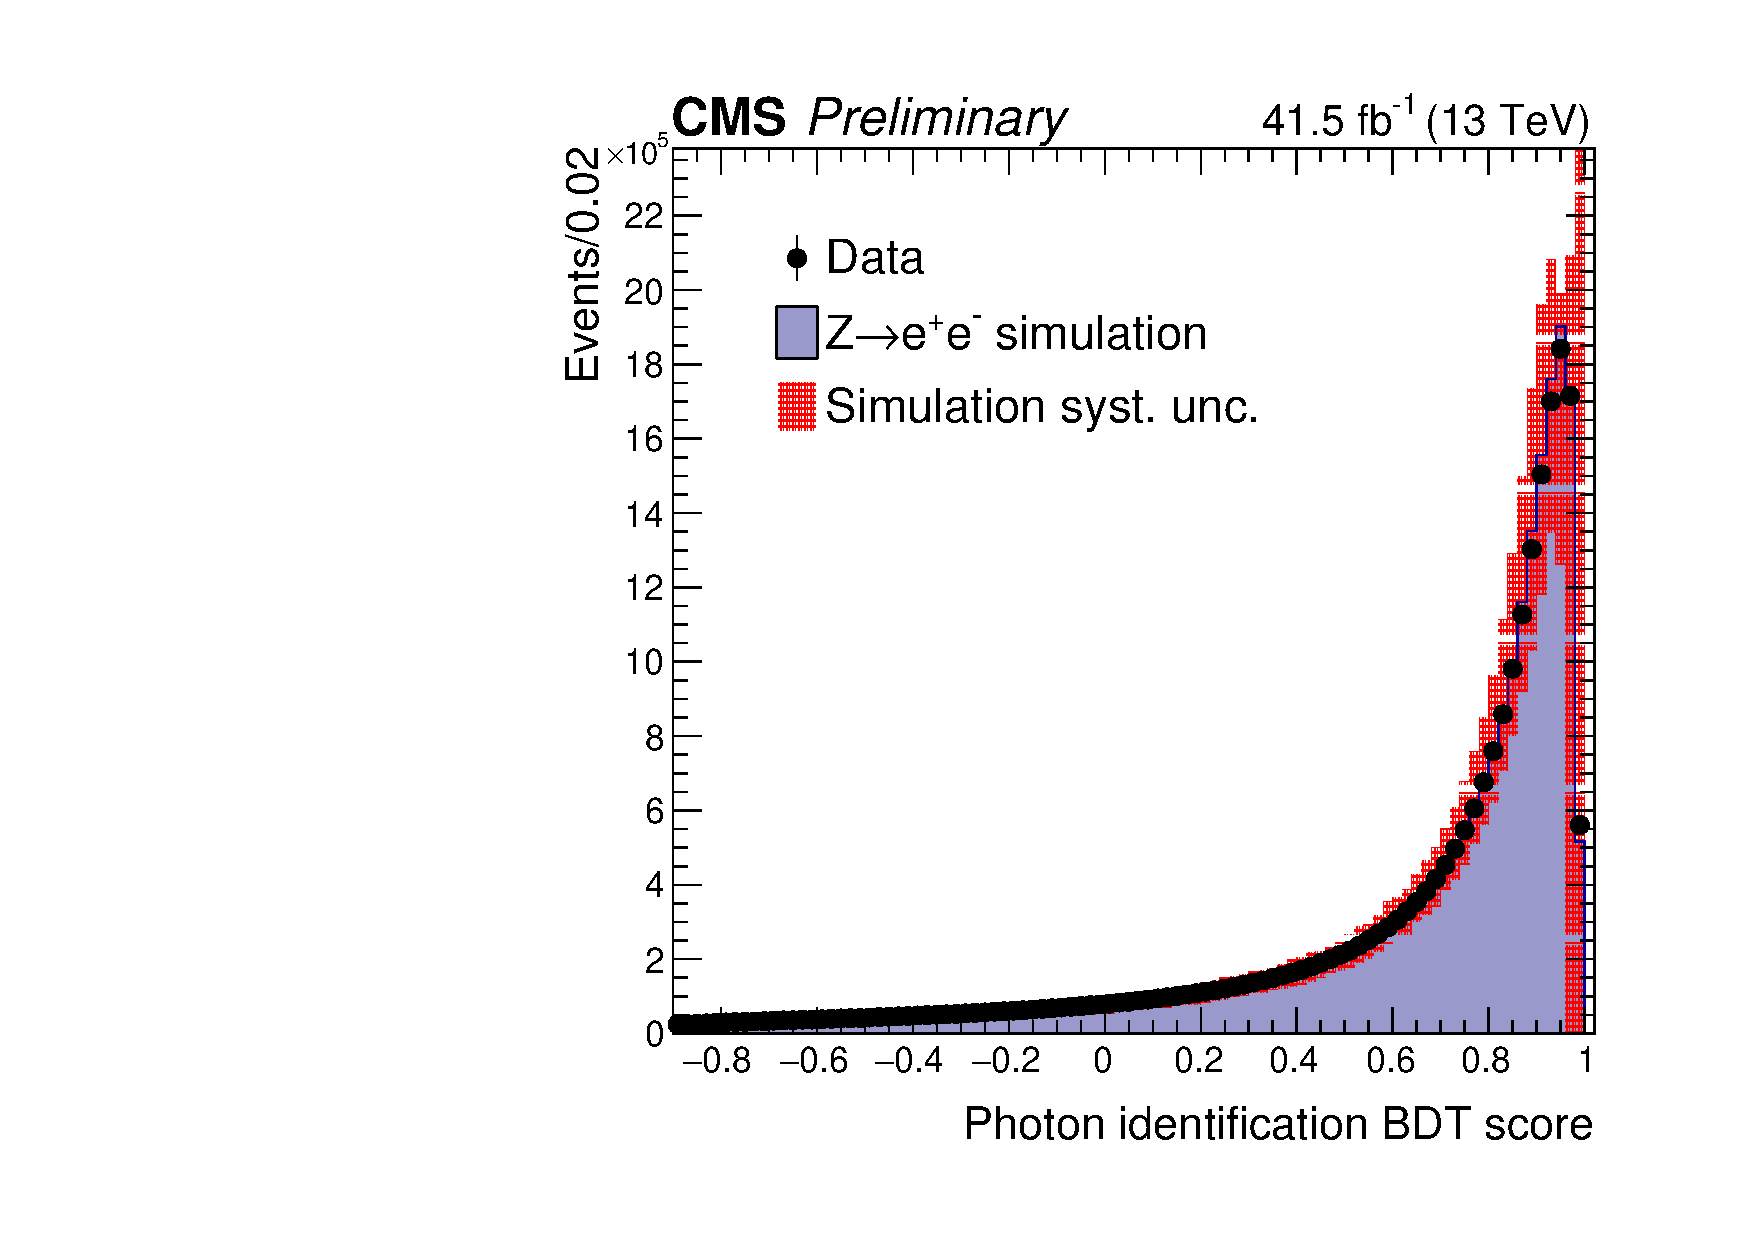
\includegraphics[width=\textwidth]{Figures/Objects/IDMVAZee_2017}
    \caption{2017}
    \label{fig:obj_IDMVAZee_2016}
  \caption{Distribution of the photon identification BDT
  for \Zee events in data and simulation, where the electrons are reconstructed as
  photons. The systematic uncertainty applied to the shape from simulation (hashed region) is
  also shown.}
  \label{fig:obj_IDMVAZee}
  \end{subfigure}
\end{figure}

\section{Vertex reconstruction}

The determination of the primary vertex from which the two photons
originate has a direct impact on the diphoton invariant mass resolution.
If the position along the beam axis ($z$) of the interaction producing
the diphoton is known to better than about \SI{1}{cm}, the invariant mass
resolution is dominated by the photon energy resolution.
For comparison, the distribution in $z$ of the position of the vertices reconstructed
from the observed tracks has an \textsc{RMS} spread of about \SI{3.4}{cm}.

\subsection{Vertex selection}

The diphoton vertex assignment relies on a BDT (the vertex identification BDT)
whose inputs are observables related to tracks
recoiling against the diphoton system:
\begin{itemize}
        \item $\sum_{i}|\vec{\pt^{i}}|^{2}$,
        \item $\displaystyle -\sum_{i}(\vec{\pt}^{i}\cdot \frac{\vec{\pt}^{\gamma\gamma}}{|\vec{\pt}^{\gamma\gamma}|})$,
        \item $(|\sum_{i}\vec{\pt}^{i}| - \pt^{\gamma\gamma})/(|\sum_{i}\vec{\pt}^{i}| + \pt^{\gamma\gamma})$,
\end{itemize}
where $\vec{\pt}^{i}$ is the transverse momentum of the $i$-th track
associated with a given vertex and $\vec{\pt}^{\gamma\gamma}$ is the
transverse momentum of the diphoton system. The sum runs over all
charged particle flow candidates associated with the given vertex.\\
In the presence of tracks from photons converted in the tracker material,
two additional input variables are used:
\begin{itemize}
        \item the number of conversions,
        \item the pull $|z_{\text{vtx}} - z_e| /\sigma_{z}$ between the
                longitudinal position of the reconstructed vertex,
                $z_{\text{vtx}}$, and the longitudinal position of the
                vertex estimated using conversion track(s), $z_e$,
                where the variable $\sigma_{z}$ denotes the uncertainty 
                on $z_e$.
\end{itemize}

\begin{figure}[h!]
  \centering
  \begin{subfigure}{0.45\textwidth}
    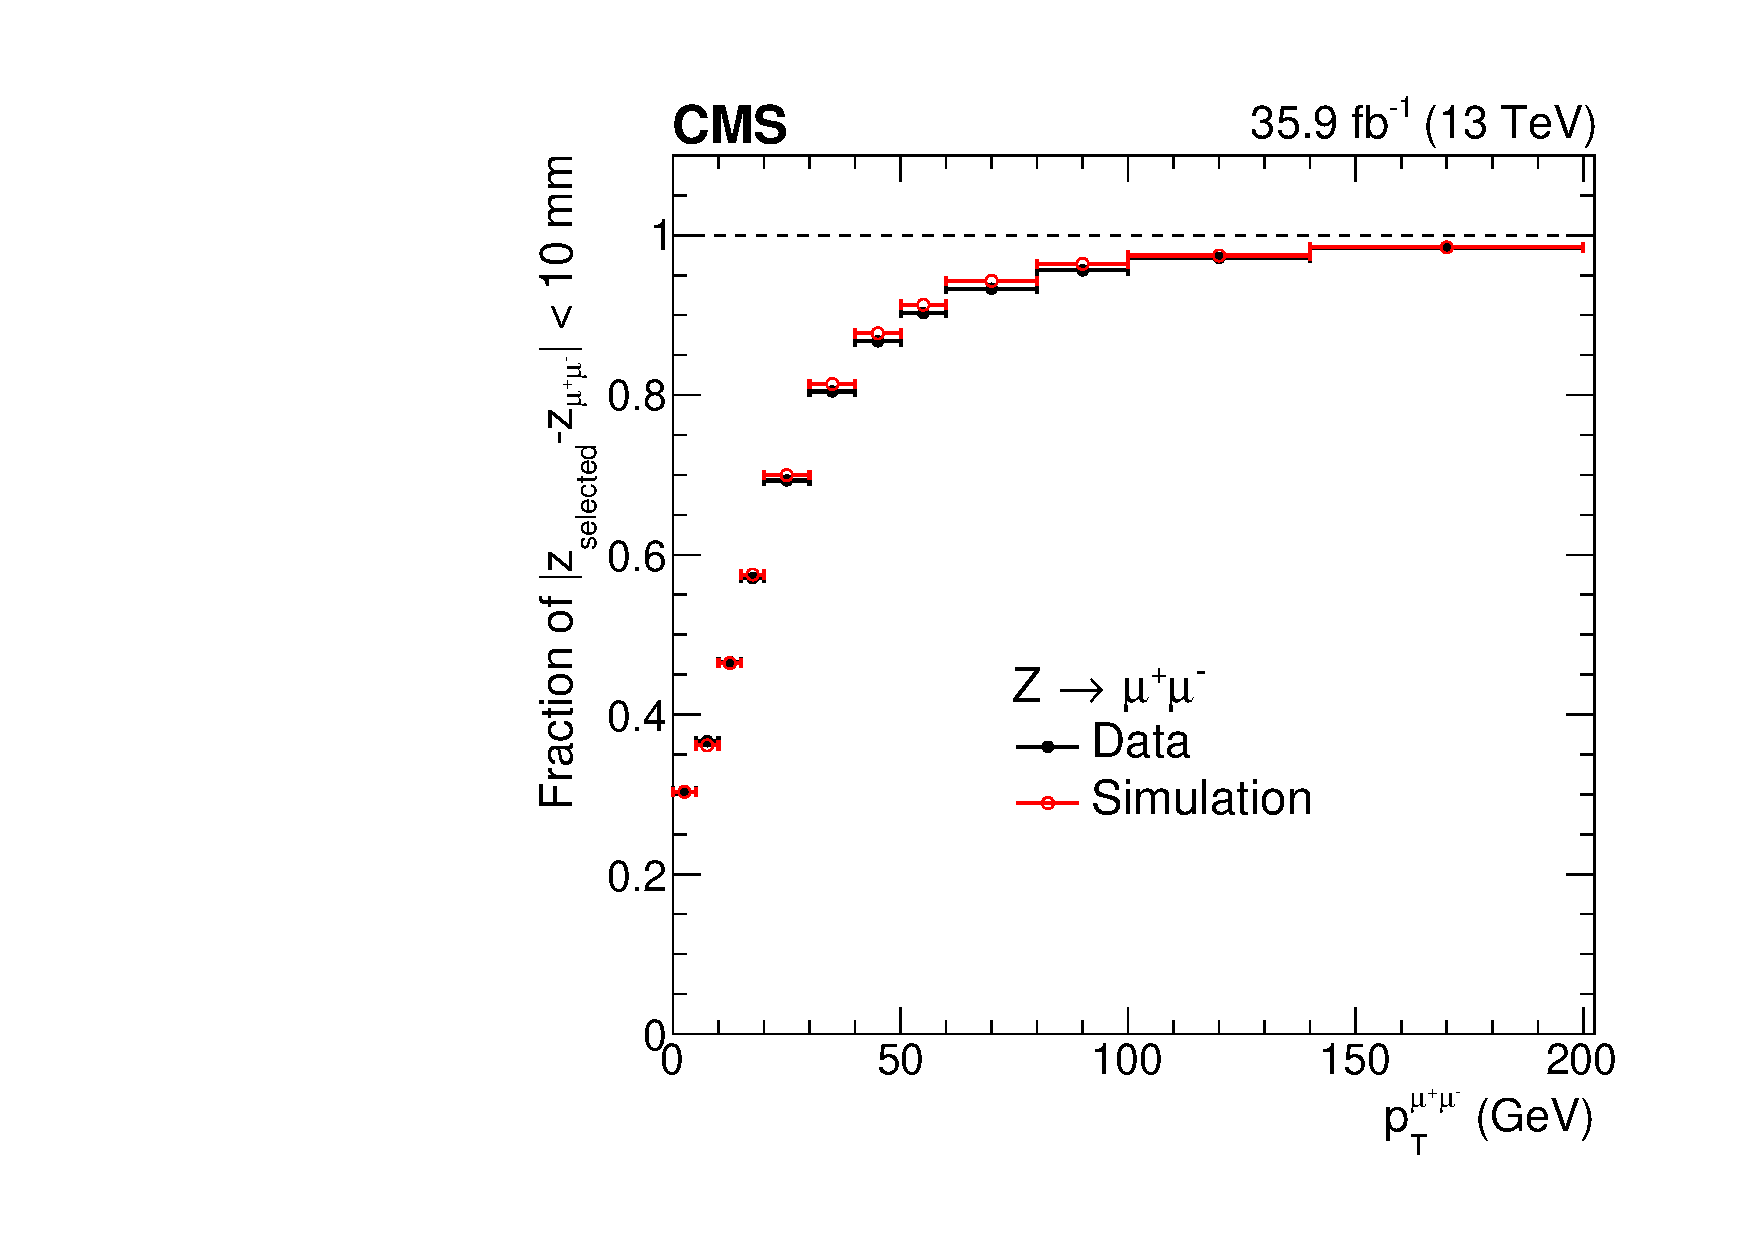
\includegraphics[width=\textwidth]{Figures/Objects/vtxid_2016}
    \caption{2016}
    \label{fig:obj_vtxid_2016}
  \end{subfigure}
  \begin{subfigure}{0.45\textwidth}
    \includegraphics[width=\textwidth]{Figures/Objects/vtxid_2017}
    \caption{2017}
    \label{fig:obj_vtxid_2016}
  \caption{
  Validation of the \Hgg vertex identification algorithm on \Zmumu events
  omitting the muon tracks. Simulated events are weighted to match the distributions of pileup
  and location of primary vertices in data.
  }
  \label{fig:obj_vtxid}
  \end{subfigure}
\end{figure}

\subsection{Vertex probability}

A second vertex-related multivariate discriminant (vertex probability BDT),
is designed to estimate, event-by-event, the probability for the vertex
assignment to be within \SI{1}{cm} of the diphoton interaction point.
%It is hereafter labelled as $\t
%ext{BDT}_{\text{VTX PROB}}$.
%This, in conjunction with the event-by-event estimate of the energy
%resolution of each photon, is used to estimate the diphoton mass
%resolution, which is then used to classify events (see
%Section~\ref{sec:classification}).
The vertex probability BDT is trained on simulated $\Hgg$ events using
the following input variables:
\begin{itemize}
        \item the number of vertices in each event,
        \item the values of the vertex identification BDT score for
                the three most probable vertices in each event,
        \item the distances between the chosen vertex and the second and
                third choices,
        \item the transverse momentum of the diphoton system, $\pt^{\gamma\gamma}$,
        \item the number of photons with an associated conversion track.
\end{itemize}

%The per-event probability to choose the vertex within 1\cm of the true
%one is parametrized as a function of the $\text{BDT}_{\text{VTX PROB}}$
%output with a $4^{th}$ order
%polynomial separately for converted and unconverted photons.

The performance of the vertex identification BDT is
validated using $\Zmumu$ events (Figure~\ref{fig:obj_vtxid}), where
the vertices are refitted, with the muon tracks omitted from the fit to
mimic a diphoton system.
In addition, the
use of tracks from converted photons to locate the vertex is validated
using $\gamma\,+\,\textrm{jet}$ events. Discrepancies between data and simulation are
corrected for in the analysis and a systematic uncertainty is introduced by
varying the ratio of data and simulation within their uncertainties.

In the simulated samples the width of the beam spot 
was about a factor 1.5 larger than
what was subsequently observed in data. To correct for this,
simulated events in which the selected vertex is more than /SI{0.1}{cm}
away from the generated one are weighted such that the width of the
distribution of the primary vertices is the same as the beam spot
 width in data.

The efficiency of correctly assigning the diphoton to be within
\SI{1}{cm} of the true vertex in $\Hgg$ simulated events is shown in
Figure~\ref{fig:obj_vtxprob} as a function of the \pt of the diphoton
pair and as a function of the number of primary vertices in the event.
The inclusive efficiency is about 81\%.

\begin{figure}[h!]
  \centering
  \begin{subfigure}{0.45\textwidth}
    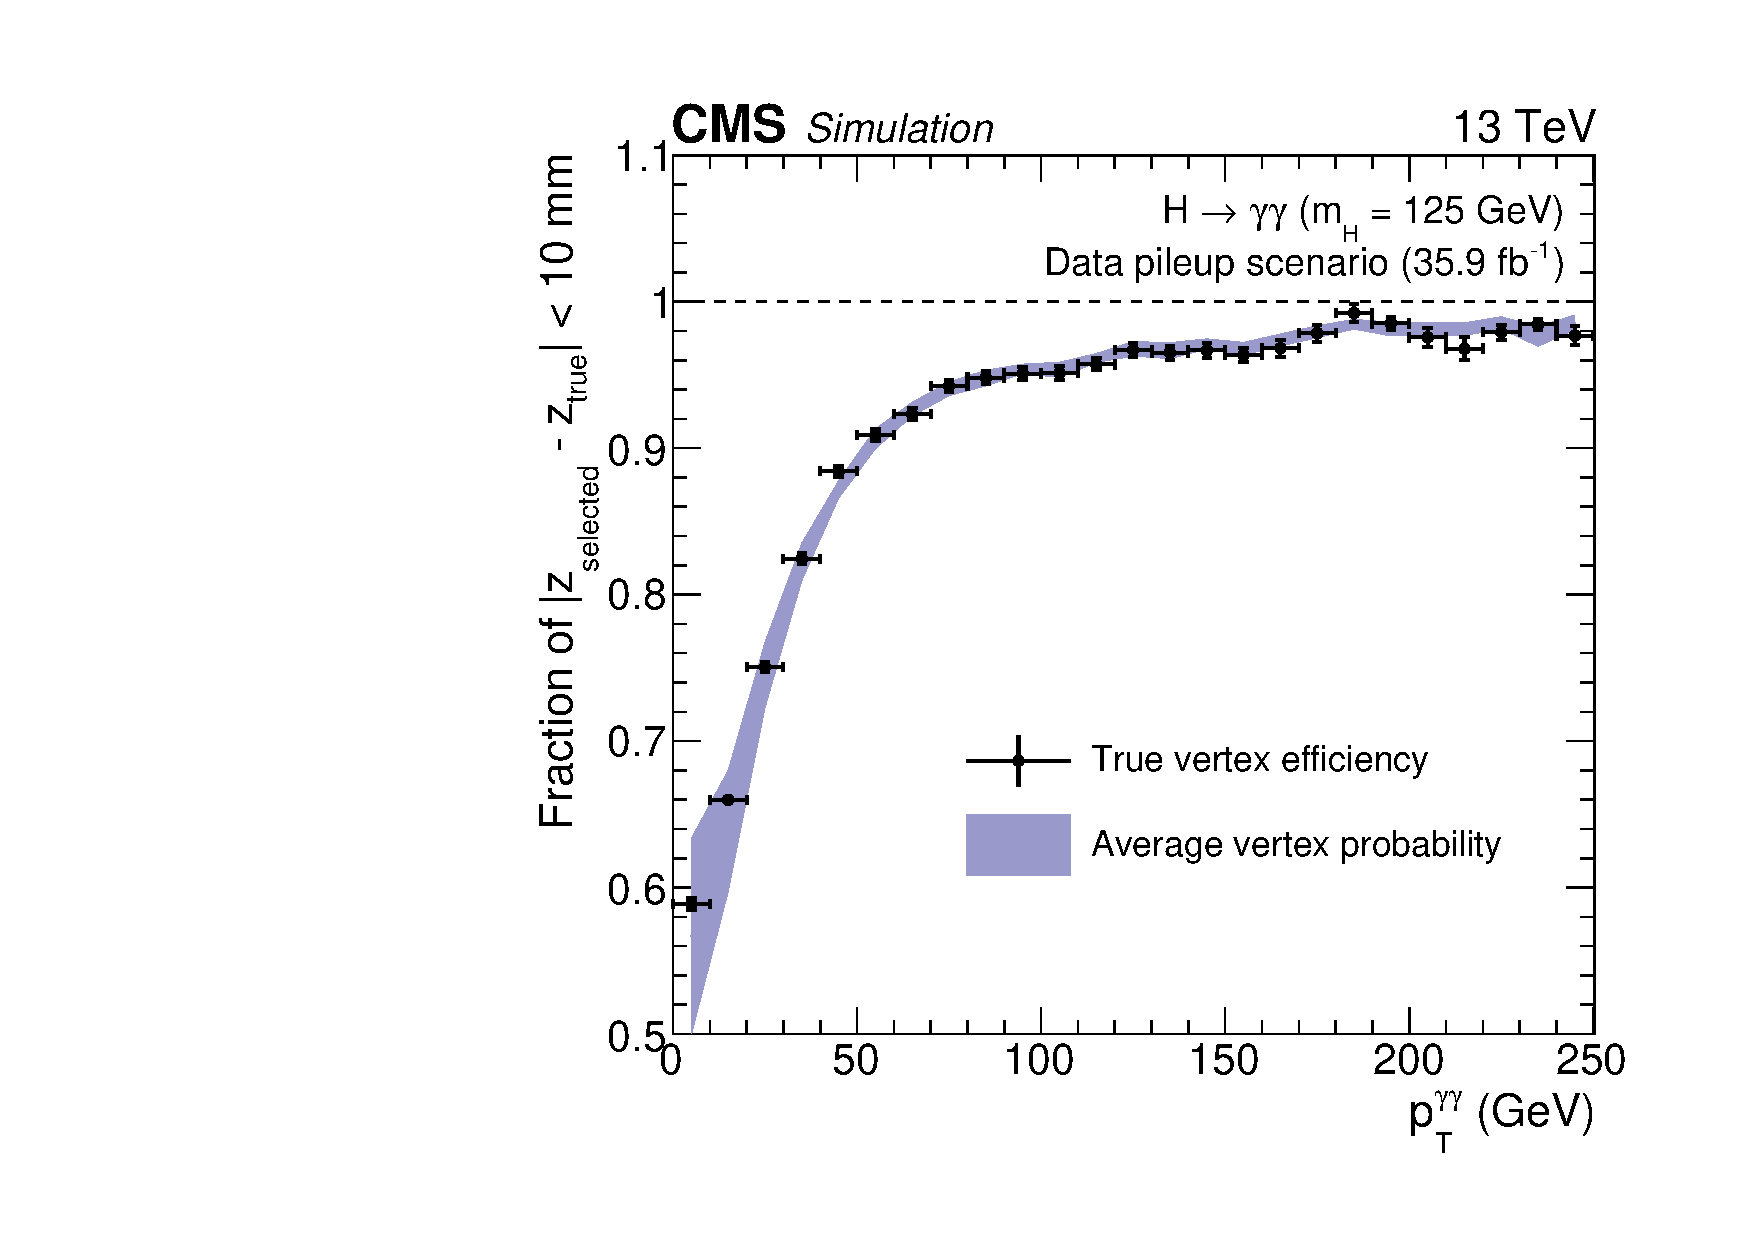
\includegraphics[width=\textwidth]{Figures/Objects/vtxprob_vspt}
    \label{fig:obj_vtxprob_vspt}
  \end{subfigure}
  \begin{subfigure}{0.45\textwidth}
    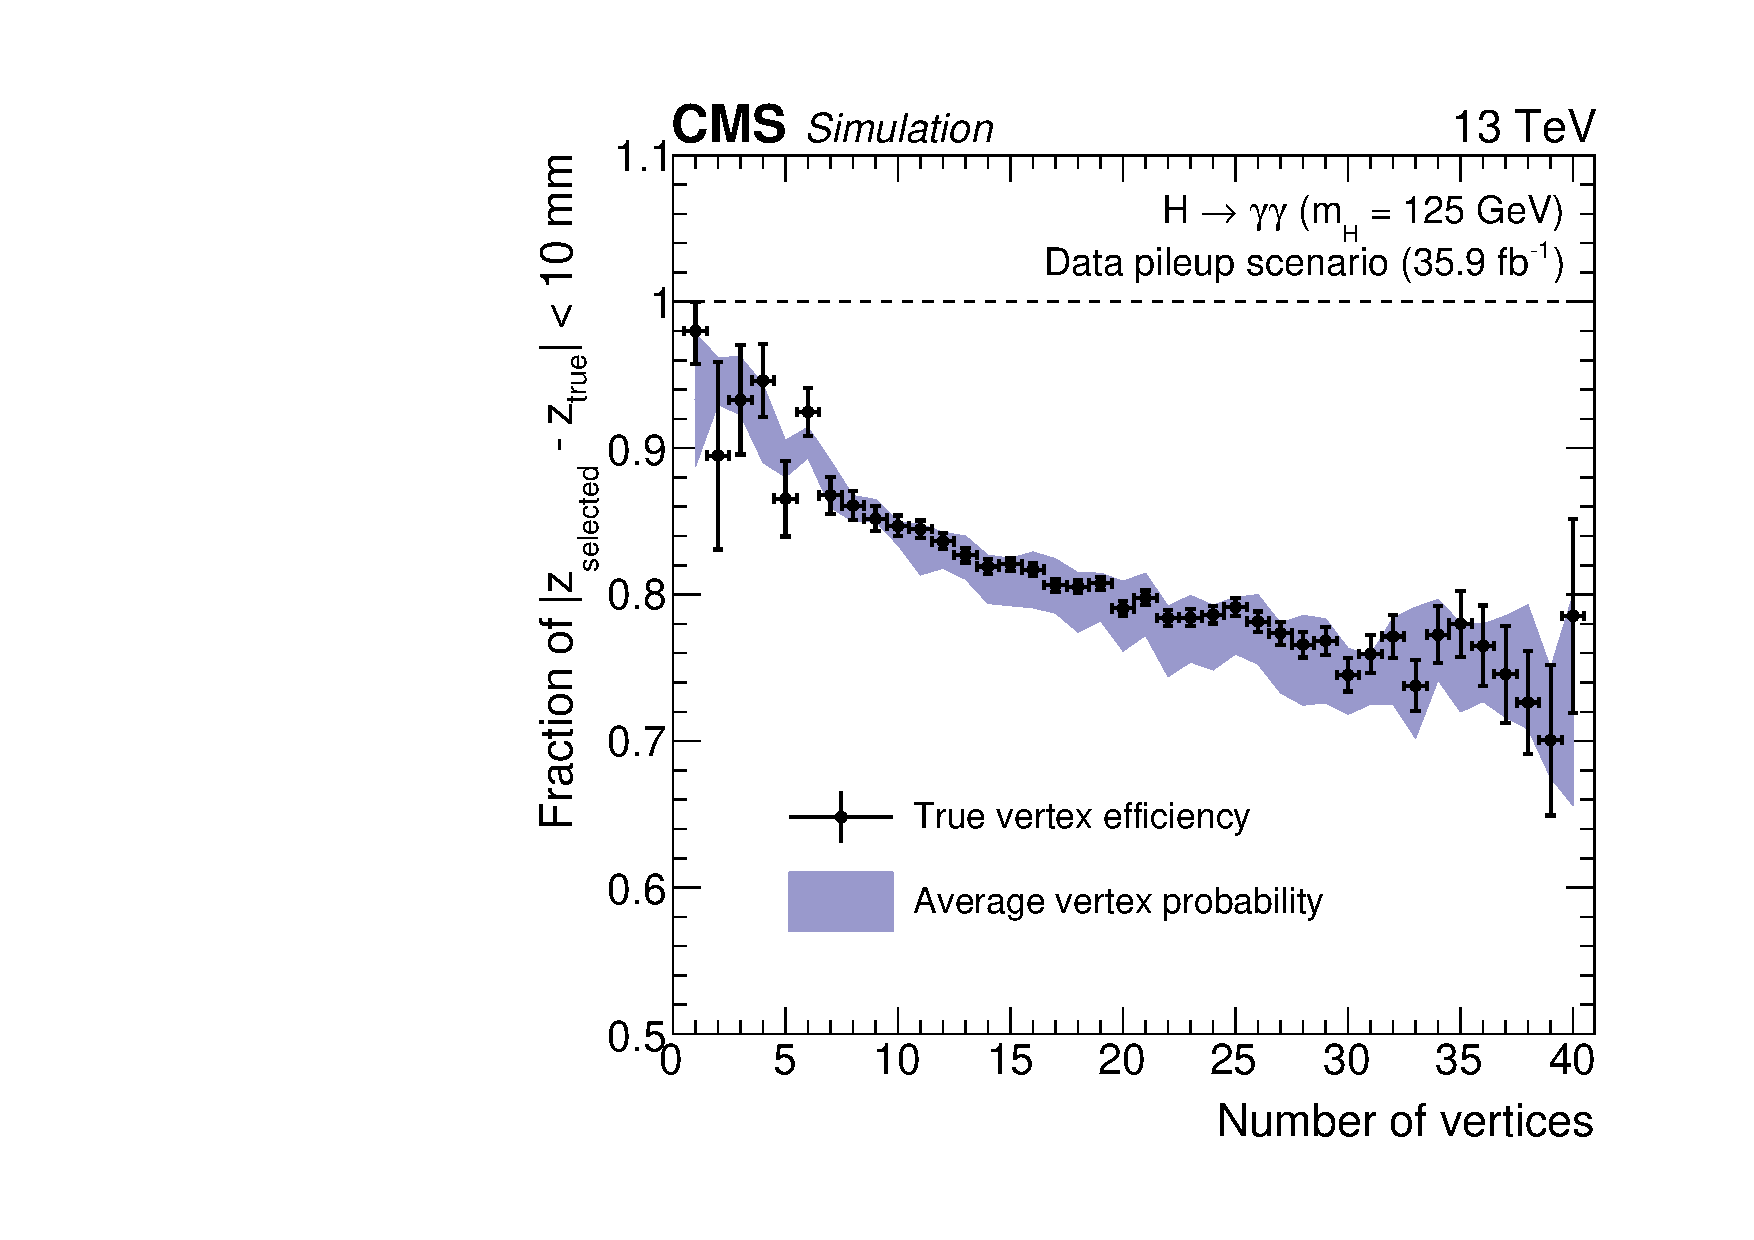
\includegraphics[width=\textwidth]{Figures/Objects/vtxprob_vsnvtx}
    \label{fig:obj_vtxprob_vsnvtx}
  \caption{
  Comparison of the true vertex identification efficiency and the average estimated
  vertex probability as a function of the reconstructed diphoton \pt (left) and of the number of
  primary vertices (right) in simulated \Hgg events with $\mH = \SI{125}{GeV}$. Events are weighted
  according to the cross sections of the different production modes and to match the distributions
  of pileup and location of primary vertices in data.
  }
  \label{fig:obj_vtxprob}
  \end{subfigure}
\end{figure}

\section{Jet reconstruction}

\section{Reconstruction of other objects}
\subsection{Electrons}
\subsection{Muons}
\subsection{Taus}
\subsection{Missing energy}
